\documentclass{article}
\usepackage[utf8]{inputenc}
\usepackage{amsmath}
\usepackage{amsfonts}
\usepackage{graphicx}

\title{Written Assignment Unit 5\\
Math 1201- College Algebra.
}
\author{Instructor - Casmir Onyeneke}
\date{October 2021}


\begin{document}

\maketitle

\section*{Question 1}
A retirement account is opened with an initial deposit of \$8,500 and earns 8.12\% interest compounded monthly. What will the account be worth in 20 years? What if the deposit were compounded monthly with simple interest? Could you see the situation in a graph? From what point one is better than the other?\\
\\\title\textbf{SOLUTION}
$${A=P\left(1+\frac{r}{n}\right)^{nt}}$$
where, 
\begin{itemize}
    \item A(t) is the value of the account including interest.
    \item P is the principal value or initial value = \$8,500.
    \item r is the annual interest rate(8.12\% or 0.0812 in decimal form).
    \item n is the frequency of the calculation in relation to t (12 months per year).
    \item t is the timespan of the calculation (20 years).
\end{itemize}
    So, therefore
    $${A = 8500\left(1 + \frac{0.0812}{12}\right)^{12\times20}}$$
    $${A = 8500 (1 + 0.00677)^{240}}$$
    $${A = 42,922.27}$$
    
    Calculation of Deposit using simple interest 
    $${A = P (1 + rt)}$$
    $${A = 8500 (1 + 0.0812 \times 20)}$$
    $${A = 8500 \times 2.624}$$
    $${A = 22,304}$$


\section*{Question 2}
Graph the function ${f(x) = 5(0.5)^{-x}}$ and its reflection about the line $y = x$ on the same axis, and give the x-intercept of the reflection. Prove that ${a^x = e^{xlna}}$. [Suggestion: type
${y= 5(0.5)^{-x} \{-7<x<2\} \{0<y<7\}}$ in desmos, and then type its inverse function]\\ 
\\\title\textbf{SOLUTION}\\
given $${a^x = e^{xlna}}$$
$${y= 5(0.5)^{-x}}$$
$${y= 5e^{-xln0.5}}$$
Taking the natural log of both sides of the equation,
$${ln\frac{y}{5}=-xln0.5}$$
Making x the subject
$${x=-\frac{ln\frac{y}{5}}{ln 0.5}}$$
swapping y with x
$${y=-\frac{ln\frac{x}{5}}{ln 0.5}}$$
The graph is shown below\\
\\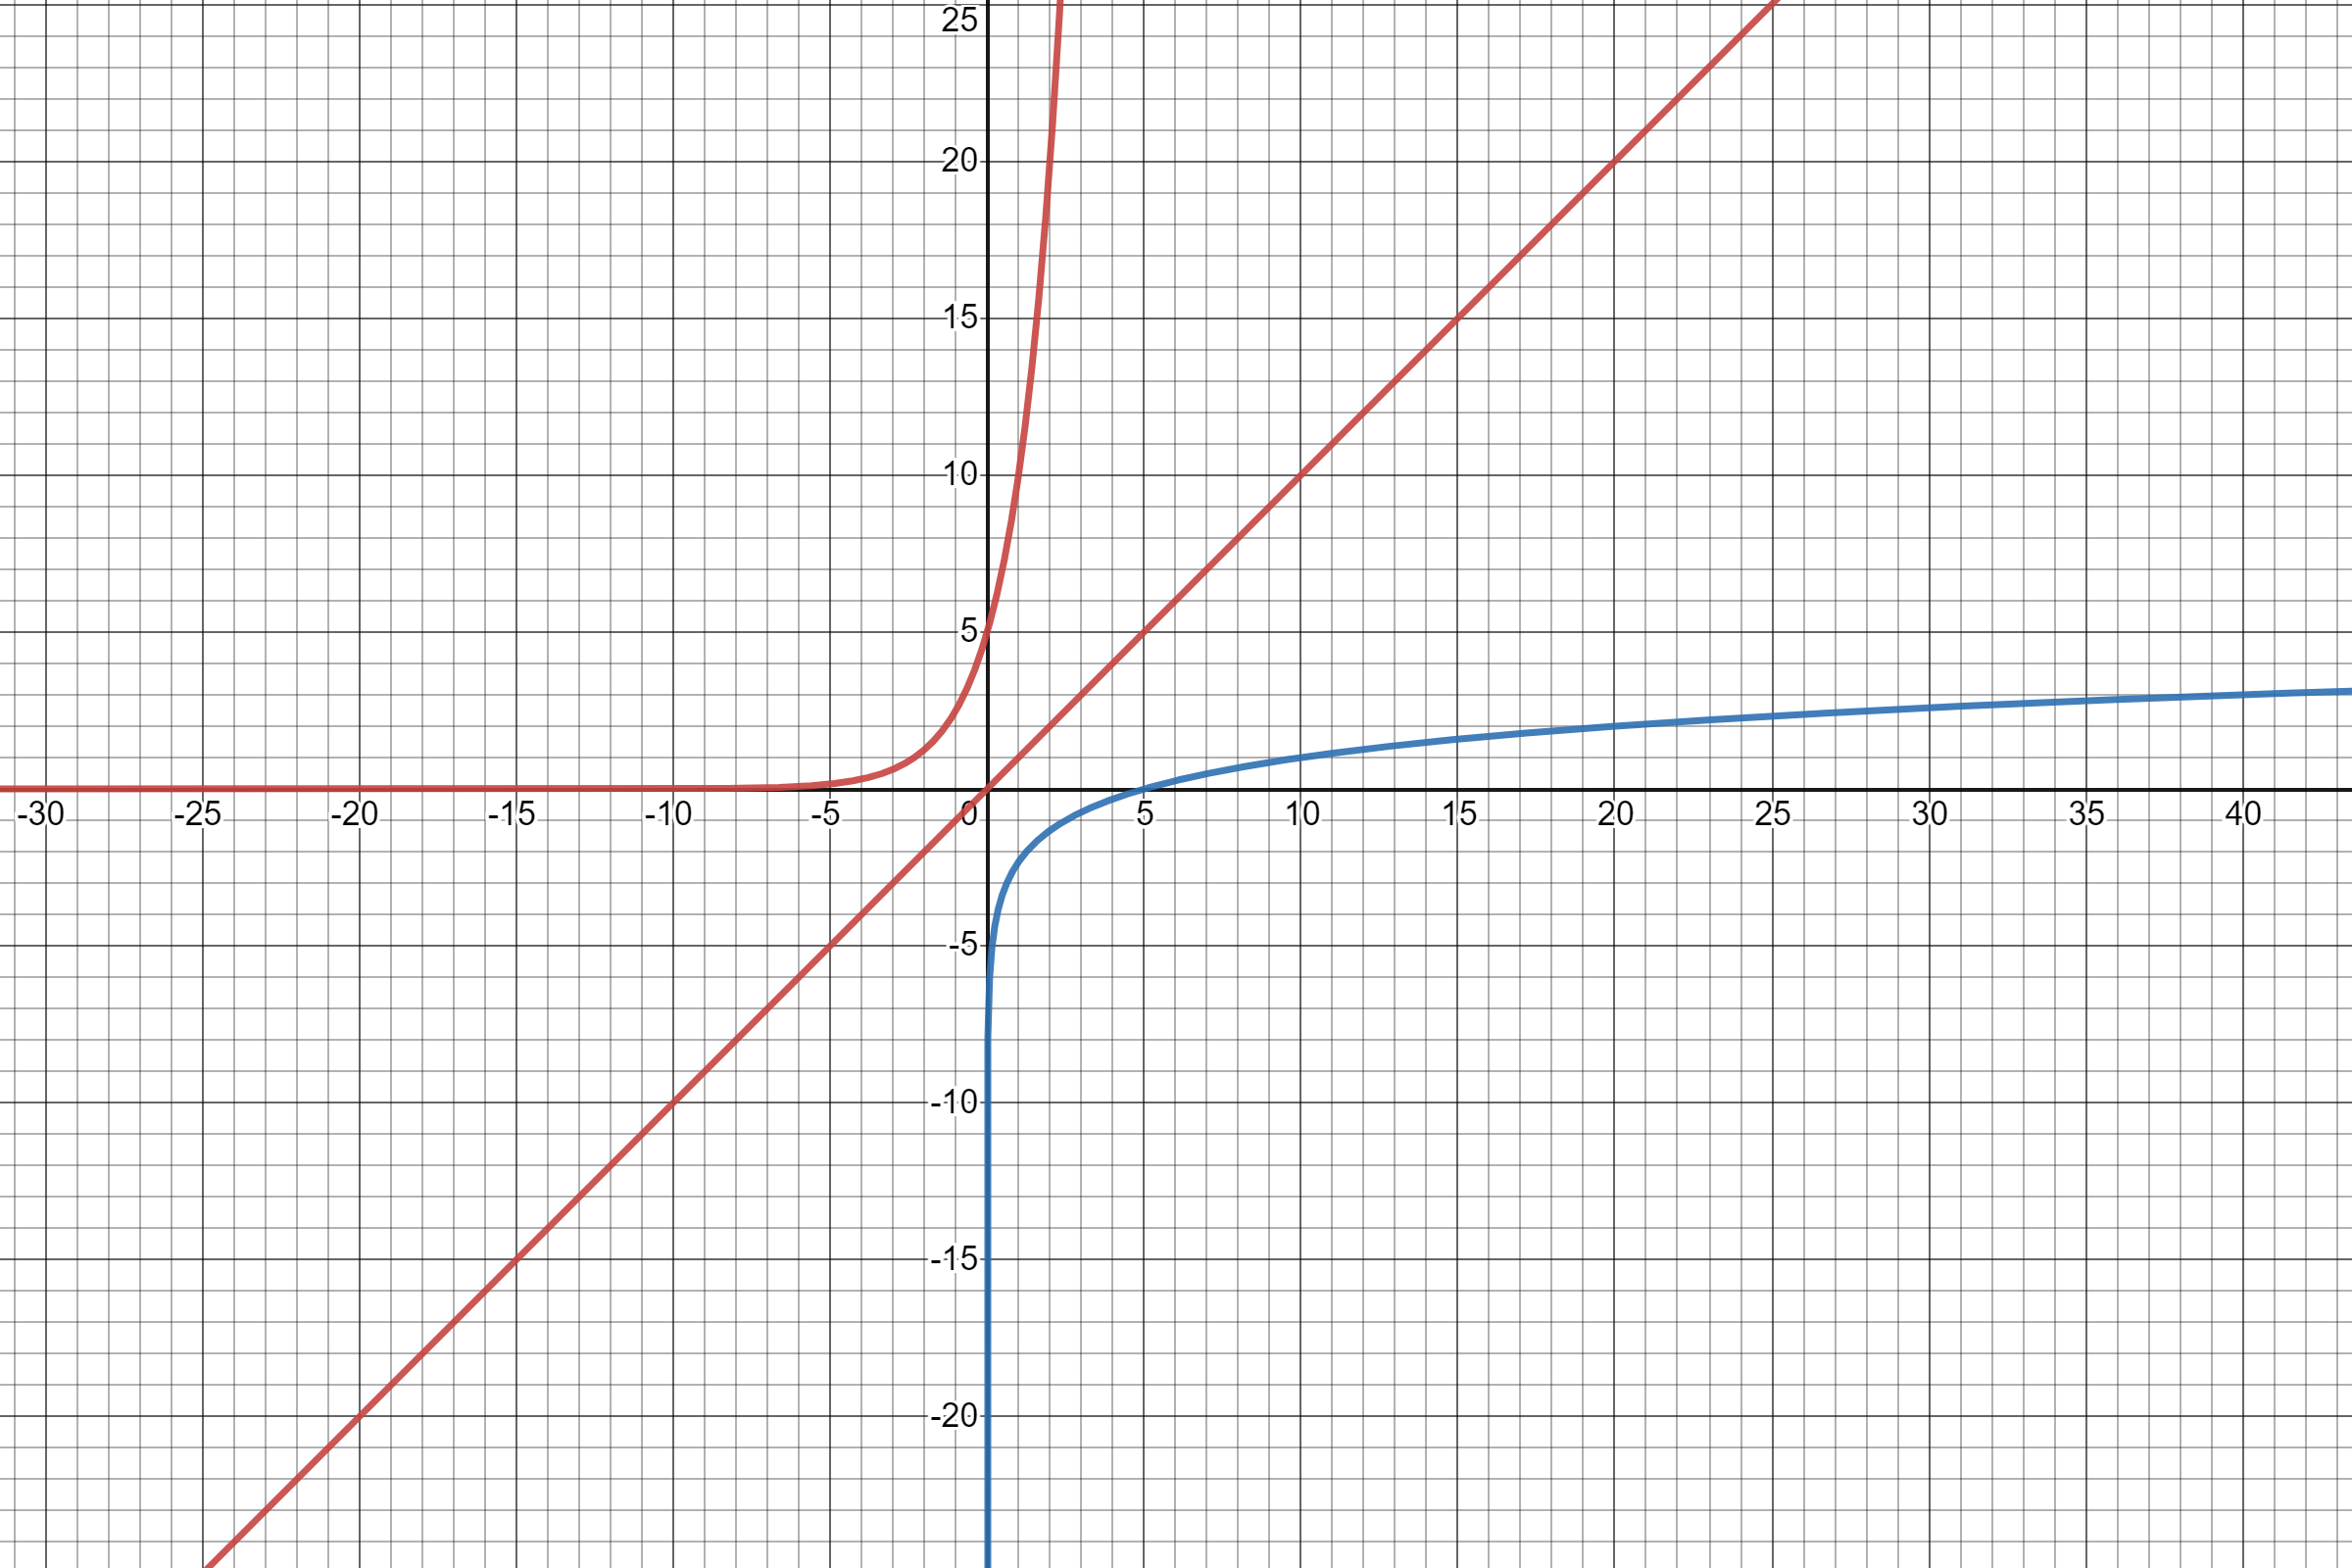
\includegraphics[scale = 0.15]{Q2}\\


\section*{Question 3}
How long will it take before twenty percent of our 1,000-gram sample of uranium-235 has decayed?\\
The decay equation is ${A(t) = A_{0}e^{kt}}$, where t is the time for the decay, and K is the characteristic of the material. Suppose T is the time it takes for half of the unstable material in a sample of a radioactive substance to decay, called its half-life. Prove that $K = \frac{ln 0.5}{T}$. What is K for the uranium-235? show the steps of your reasoning.\\
\\\title\textbf{SOLUTION}\\
T= half life of uranium-235 = 703,800,000 years
$${800 = 1000e^{\frac{ln0.5}{703800000}t}}$$
Dividing through by 1000
$${0.8 = e^{\frac{ln0.5}{703800000}t}}$$
taking the natural log of both sides
$${ln 0.8 = \frac{ln0.5}{703800000}t}$$
Dividing through by  ${\frac{ln0.5}{703800000}}$
$${t = 703800000\times\frac{ln 0.8}{ln0.5}}$$
$${t = 703800000\times0.321928}$$
$${t = 226,572,993}$$
For the constant K
$${A(t) = A_{0}e^{Kt}}$$
$${\frac{A_{0}}{2} = A_{0}e^{KT}}$$
$${\frac{1}{2} = e^{KT}}$$
$${ln0.5 = {KT}}$$
$${K = \frac{ln0.5}{T}}$$

For K in the Uranium-235, we have
$${K = \frac{ln0.5}{T}}$$
$${K = \frac{ln0.5}{703,800,000}}$$
$${K = \frac{1}{100,000,000}\times\frac{ln0.5}{7}}$$
$${K = \frac{1}{100,000,000}\times-0.099021026}$$
$${K = \frac{1}{100,000,000}\times-0.1}$$
$${K = -10^9}$$
\section*{REFERENCES}
Abramson, J. (2017). \textit{Algebra and trigonometry}. OpenStax, TX: Rice University. Retrieved
from https://openstax.org/details/books/algebra-and-trigonometry
\end{document}